\documentclass[conference,letterpaper]{IEEEtran}
\usepackage[T1]{fontenc}
\usepackage{newtxtext,newtxmath}
\usepackage{graphicx}
\usepackage{booktabs,array}
\usepackage{amsmath}
\usepackage[hyphens]{url}
\usepackage[hidelinks]{hyperref}
\graphicspath{{figures/}}
\newcommand{\ch}{\operatorname{Compute}_{95}}
\newcounter{algorithm}
\newcolumntype{L}[1]{>{\raggedright\arraybackslash}p{#1}}
\hyphenation{ChiaLoop MediumBOOM}
\begin{document}

\title{Adaptive ChiaLoop for Compute-Efficient\\
Coverage Closure in Chip Verification}
\author{\IEEEauthorblockN{Kapil Bansal \qquad Khushal Sethi}
\IEEEauthorblockA{CHIA Hackathon at A3@MICRO 2026\\
Artifact: \url{https://github.com/kbansal1512/chia-hackathon}}}
\maketitle

\begin{abstract}
Chip verification must close coverage within compute, license, and schedule budgets, yet fixed schedules can continue spending resources on low-yield work. We present ChiaLoop, an adaptive chip-verification system that replans job allocation using observed coverage gain per compute-hour. Its policy aims to exploit the nonlinear effects of scenario selection by prioritizing high-yield obligations and avoiding jobs proven unable to contribute under registered assumptions. In an exploratory post-saturation comparison across five MediumBOOM trial pairs, Adaptive recorded 169.2 mean new-bin hits per trial versus 160.6 for a fixed 4:1 constrained-random-to-directed schedule. This preliminary result motivates broader evaluation. ChiaLoop is designed to coordinate allocation and budgets across users, chip configurations, license constraints, and AI agents.
\end{abstract}

\begin{IEEEkeywords}
adaptive verification, coverage closure, resource allocation, constrained-random verification, formal verification, CHIA
\end{IEEEkeywords}

\section{Introduction}
Verification allocates limited execution capacity across complementary methods. Constrained-random tests sample diverse behaviors, directed tests concentrate on specific scenarios, and formal queries produce witnesses or establish unreachability under explicit assumptions. Their usefulness changes with the remaining obligations. An allocation effective early in a campaign can become wasteful near its closure target.

Coverage-directed test selection has demonstrated the value of using feedback to prioritize simulation work~\cite{masamba}. A broader campaign also chooses among verification engines and coverage partitions. The resulting question is operational: given the current evidence and available resources, which eligible job should receive the next compute slot? Increasing parallelism alone does not resolve this choice. It may shorten elapsed time while executing the same amount of redundant work.

We propose \emph{ChiaLoop}, a verification controller hosted on the CHIA execution framework~\cite{chia}. ChiaLoop treats the campaign objective as an explicit input. In the core study, the objective is to reduce occupied compute-hours required to reach a registered sound-closure target. The controller measures the marginal closure obtained from completed jobs, updates recent yield estimates, and selects further work subject to compute and license constraints. Its control decisions depend on observed outcomes rather than fixed coverage-percentage thresholds for switching engines.

The research question is: \emph{Does completion-driven allocation across constrained-random, directed, and formal work reach 95\% sound coverage closure using fewer compute-hours than a fixed hybrid schedule, when jobs, resources, and evidence rules are held constant?} A fixed hybrid is the primary control because it already has access to every engine used by the adaptive treatment. This comparison separates allocation quality from the benefit of adding formal or directed verification to a simulation campaign.

This paper makes three methodological contributions. First, it defines an objective and evidence model that couples compute accounting with a fixed universe of coverage obligations. Second, it specifies a deterministic adaptive policy and asynchronous execution architecture with explicit resource admission. Third, it reports an exploratory post-saturation comparison using five MediumBOOM trial pairs, with the earlier single-pair pilot and hindsight replay kept separate.

\section{Problem Formulation and Evidence Model}
\label{sec:formulation}
Let $P$ be the frozen coverage universe and $J$ the immutable job catalog. A point is open, hit, or proven unreachable; sound closure is $(|H|+|U|)/|P|$ with a fixed denominator. Simulation hits and formal outcomes must match the registered predicate and scope. Table~\ref{tab:evidence} summarizes the evidence rules.

\begin{table}[t]
\caption{Coverage Evidence and Acceptance Rules}
\label{tab:evidence}
\centering\footnotesize
\setlength{\tabcolsep}{4pt}
\begin{tabular}{@{}L{0.28\columnwidth}L{0.17\columnwidth}L{0.47\columnwidth}@{}}
\toprule
Evidence & State & Required interpretation \\
\midrule
Simulation observation & Hit & Native evidence for the registered predicate and scope. \\
Formal cover witness & Hit & Legal witness under matching model and assumptions. \\
Complete unreachability proof & Proven unreachable & Exact obligation, qualified scope, and registered assumptions. \\
Bounded non-hit; timeout; unknown; error & Open & No evidence sufficient to close the point. \\
Conflicting or incompatible result & Unchanged & Reject and log; investigate the campaign's validity. \\
\bottomrule
\end{tabular}
\end{table}

The driver derives novelty at merge time. Duplicate hits earn no credit; conflicting evidence is quarantined (Fig.~\ref{fig:evidence}).

\begin{figure}[t]
\centering
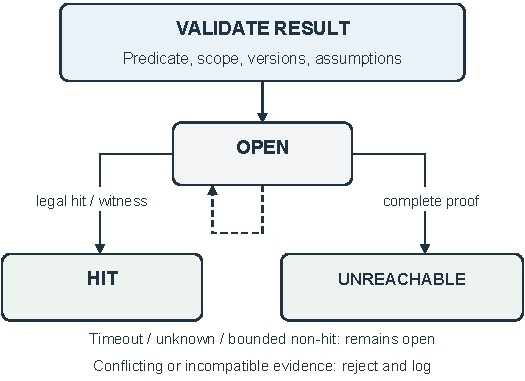
\includegraphics[width=\columnwidth]{evidence.pdf}
\caption{Evidence-governed state updates. Validation precedes every transition. Incomplete evidence leaves an obligation open; a conflicting result is quarantined without awarding additional closure.}
\label{fig:evidence}
\end{figure}

The objective is occupied slot-hours to 95\% sound closure: $Q(t)=\int_0^t\sum_s a_s(u)\,du$ and $\mathrm{Compute}_{95}=Q(T_{95})$. All occupied work, including failures and timeouts, counts toward cost.

\section{ChiaLoop Architecture and Adaptive Policy}
\label{sec:architecture}
\subsection{Separation of Policy, Execution, and Evidence}
Figure~\ref{fig:architecture} shows the proposed control path. The campaign specification fixes the objective, coverage universe, job catalog, capacities, and stopping rules. The controller owns the coverage state and yield table. A replaceable policy chooses jobs, while the dispatcher admits and launches them through three CHIA function nodes: \texttt{run\_crv}, \texttt{run\_directed}, and \texttt{run\_formal}. Each invocation executes one independently schedulable job.

\begin{figure*}[t]
\centering
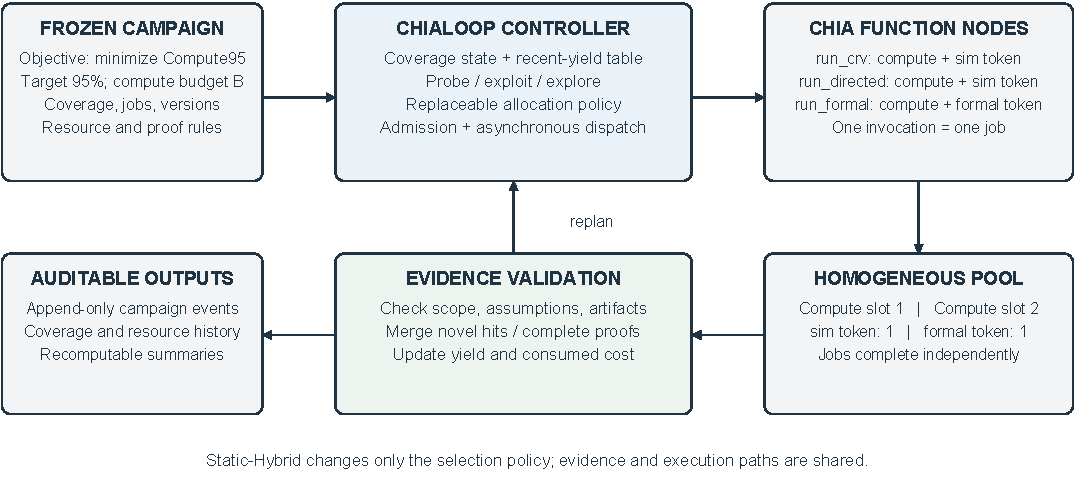
\includegraphics[width=\textwidth]{architecture.pdf}
\caption{Proposed ChiaLoop architecture and completion-driven feedback. The reported experiment shares the catalog, evidence validator, local resource admission, and event log across policy arms; it does not execute through the CHIA nodes. Resource tokens represent capacity, not physical machines.}
\label{fig:architecture}
\end{figure*}

The registered toggle campaigns contain CRV and directed simulation jobs only, with two compute slots, one simulation token, and no formal jobs. The endpoint is exact signal-toggle bits; SVA/property outcomes cannot soundly hit or retire those toggle IDs, so formal jobs are excluded rather than mixed into this comparison. A declared formal-license capacity does not imply formal work was executed. These campaign-controlled tokens express concurrency constraints; an open-source tool run does not imply possession of a commercial license.

After probing each eligible lane once, Adaptive ranks lanes by new validated points per occupied compute-hour over the last three completed jobs. Every tenth post-probe dispatch explores the least-sampled eligible lane; ties and job order are frozen. The asynchronous driver validates completions, merges unique hits, updates yield, admits work only when resource tokens fit, and records decisions and costs in an append-only event log. Static-Hybrid uses the same execution and evidence path with a fixed lane schedule.

\section{Experimental Methodology}
\label{sec:method}
\subsection{Workload and Frozen Inputs}
We use one MediumBOOM configuration~\cite{boom} and five fixed planning partitions: integer/control, load-store/ordering, multiply/divide/atomics, privilege/exceptions, and mixed long-running behavior. Inputs and coverage IDs are frozen before paired runs; duplicate point hits count once. Table~\ref{tab:config} summarizes the five-pair cohort.

\begin{table}[t]
\caption{Campaign Configuration and Experimental Controls}
\label{tab:config}
\centering\footnotesize
\begin{tabular}{@{}L{0.34\columnwidth}L{0.61\columnwidth}@{}}
\toprule
Item & Core-study specification \\
\midrule
Design and planning groups & One MediumBOOM configuration; five partitions. \\
Engines & CRV and directed simulation in the registered toggle study; formal is excluded from this endpoint. \\
Execution capacity & Two identical compute slots. \\
Admission tokens & One simulation token; no formal jobs are catalogued. \\
Closure target & 95\% of the frozen point universe. \\
Adaptive parameters & Three completed jobs per window; exploration every tenth post-probe dispatch. \\
Static manifest & Repeating 4 CRV : 1 directed schedule. \\
Pairing & Identical jobs and initial state within each pair; randomized arm order. \\
Execution registration & The frozen cohort protocol and manifests are archived with the measured results. \\
\bottomrule
\end{tabular}
\end{table}

The registered endpoint is native signal-toggle evidence; the measured toggle catalog contains CRV and directed jobs but no formal jobs. Source-line, semantic-family, and proof results are not mixed into this endpoint.

\subsection{Primary Baseline and Treatment}
Static-Hybrid follows a fixed 4 CRV:1 directed schedule; Adaptive changes only dispatch order. Each pair uses the same frozen jobs, evidence validator, initial state, resources, and stopping rule, with randomized arm order and no result replay. The comparison runs through a local asynchronous executor, not CHIA/Ray; historic proxy-meter counts are excluded.

\begin{table*}[t]
\caption{Exploratory Capped-Concurrency MediumBOOM Open-Toggle Subset (Trials 40--44).}
\label{tab:results}
\centering\small
\begin{tabular}{@{}L{0.30\textwidth}L{0.31\textwidth}L{0.31\textwidth}@{}}
\toprule
Metric & Static-Hybrid & Adaptive ChiaLoop \\
\midrule
\multicolumn{3}{l}{\textit{Five paired trials at the 0.25 compute-hour checkpoint}} \\
Summed new-bin hits across five trials$^\dagger$ & 803 & 846 \\
Mean new-bin hits per trial & 160.6 & 169.2 \\
Adaptive minus Static-Hybrid & \multicolumn{2}{L{0.62\textwidth}}{+43 summed hits; +8.6 per trial} \\
\multicolumn{3}{l}{\textit{Log projection to 200 catalogs (exploratory; not measured)}} \\
Additional residual-set closure at 200$^\ddagger$ & 11.09\% & 11.55\% \\
Adaptive relative increase over static projection & \multicolumn{2}{L{0.62\textwidth}}{+4.2\% in post-saturation incremental gain} \\
\bottomrule
\end{tabular}
\par\smallskip{\footnotesize $^\dagger$ Per-trial hit counts are summed; a toggle bin hit in multiple independent trials may be counted multiple times. These are not pooled-unique totals. $^\ddagger$ Policy-specific log extrapolations fit only to the five measured trials; they are exploratory, not observed outcomes.}
\end{table*}

\section{Results and Analysis}
\label{sec:results}
\subsection{Exploratory Capped-Concurrency Open-Toggle Comparison}
The endpoint is native Verilator signal-toggle bins left open after the prior pilot; neither the legacy 51-point proxy nor the 66 semantic families enters the denominator. This is toggle activity, not source-line or functional coverage.

Summed per-trial new-bin hits were 803 for Static-Hybrid and 846 for Adaptive, or 160.6 and 169.2 per trial; the paired summed difference was +43 hits (+8.6 per trial). The post-saturation log curves project additional residual-set closure of 11.09\% and 11.55\% at 200 catalogs, respectively, a +4.2\% relative difference in projected incremental gain. These values extrapolate from only five measured catalogs; they are exploratory projections, not observed outcomes or evidence of a confirmatory policy advantage.

Workloads are pre-generated; Adaptive changes dispatch order only and does not synthesize directed tests on the fly.

\begin{figure*}[t]
\centering
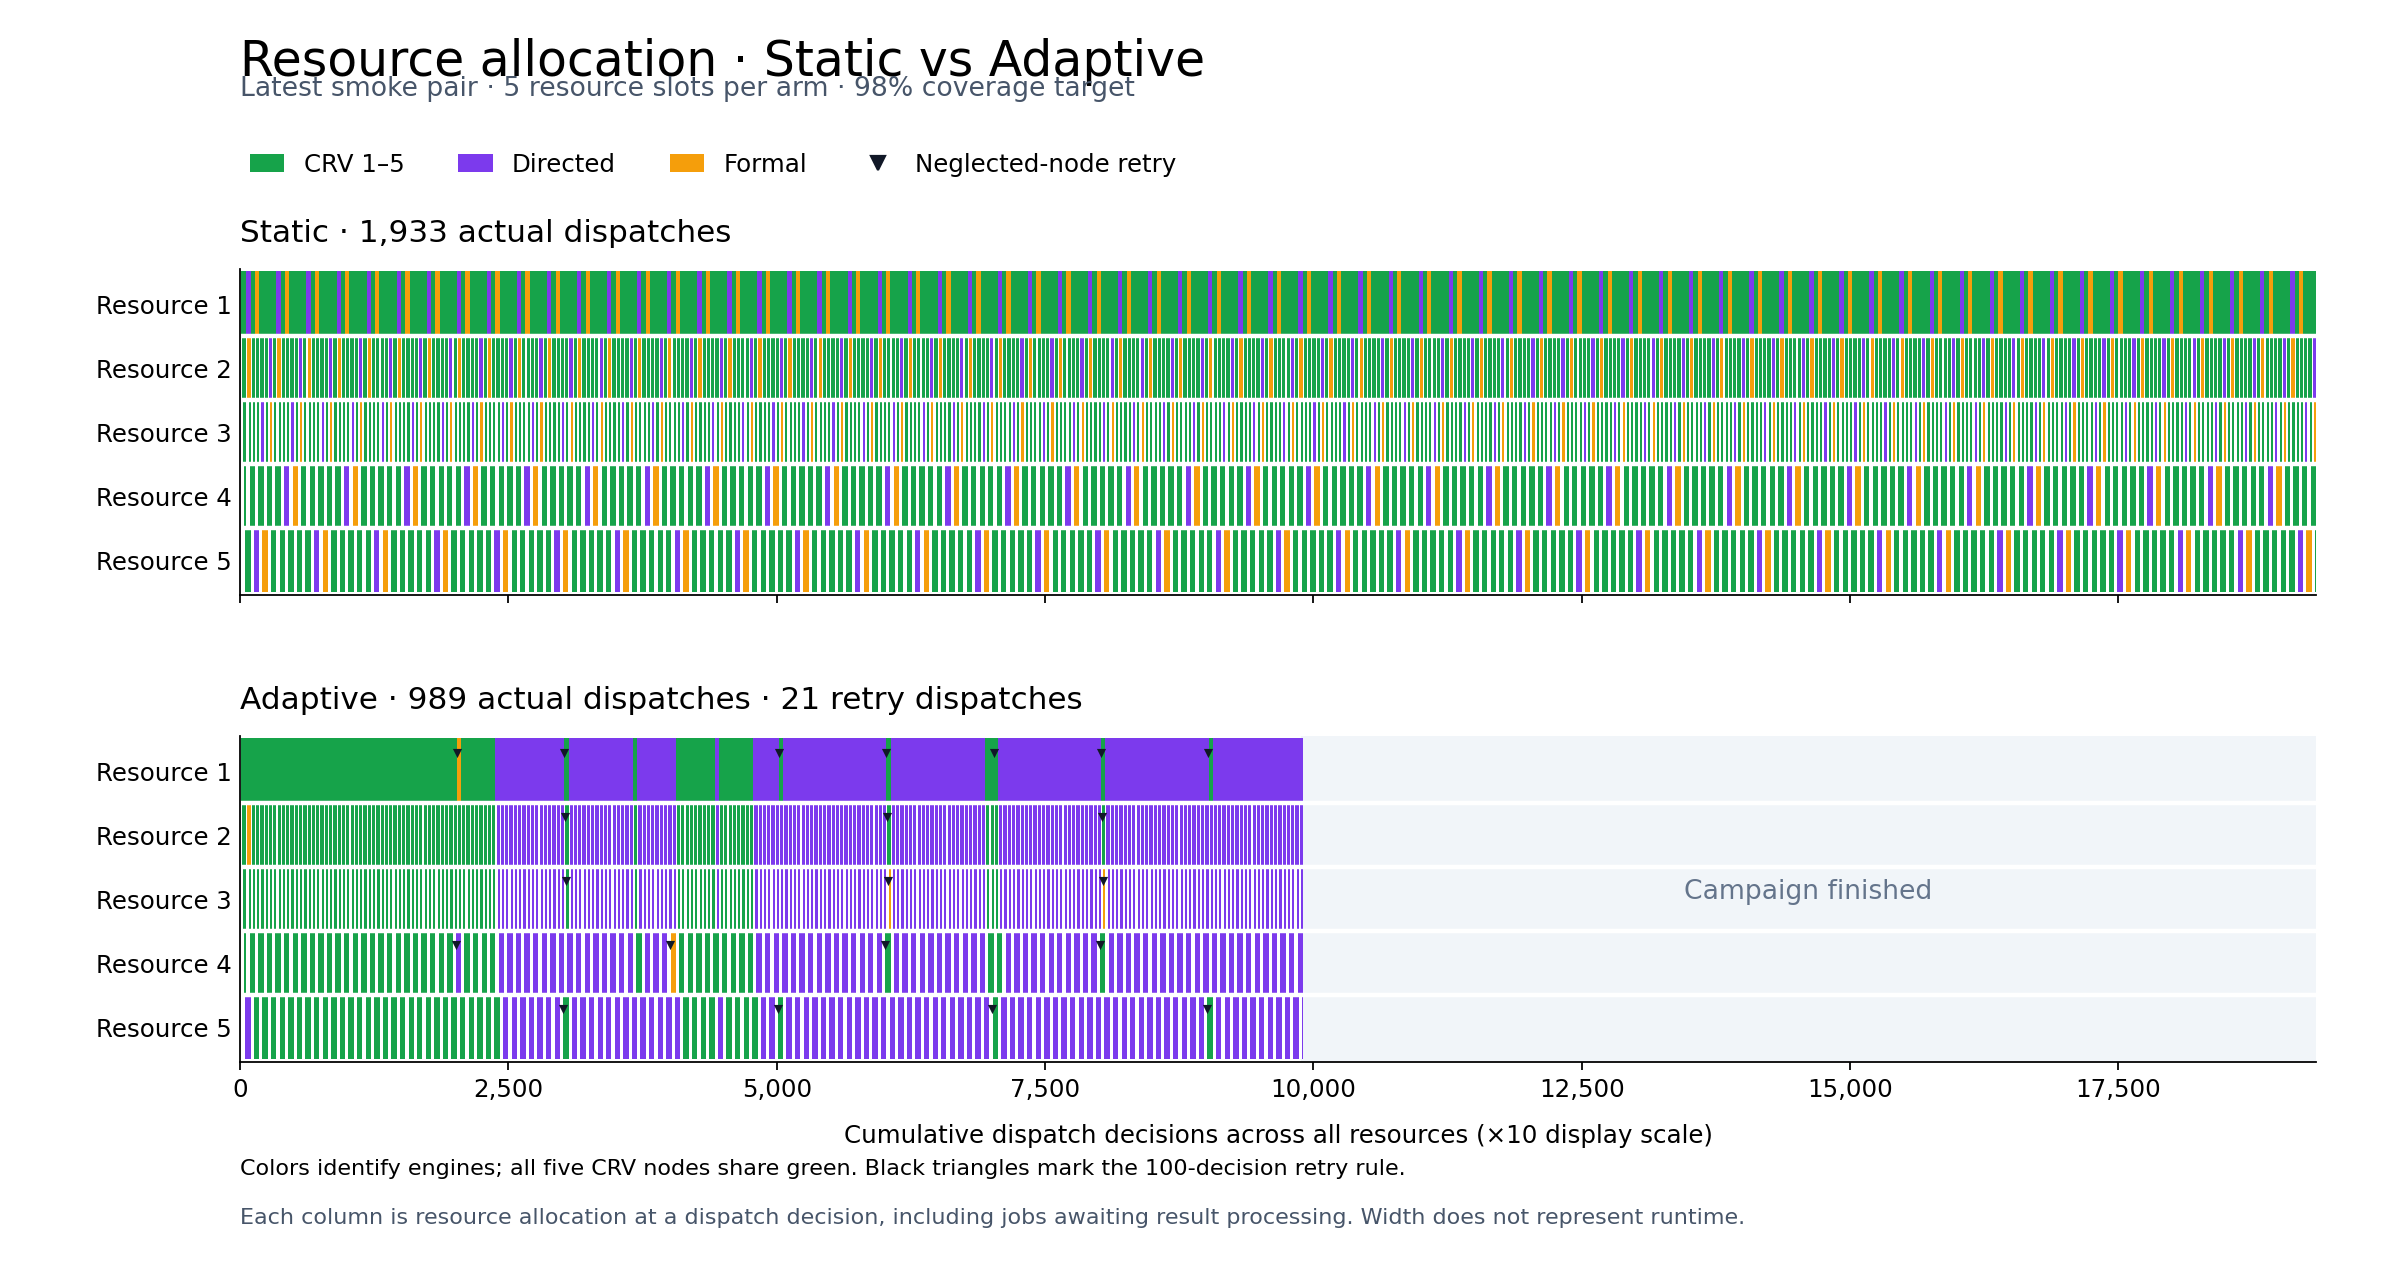
\includegraphics[width=0.92\textwidth]{resource_allocation_trace.png}\\[-1mm]
{\footnotesize (a) Illustrative static and adaptive resource allocation across five slots. This separate trace includes formal work and a 98\% target.}\\[1mm]
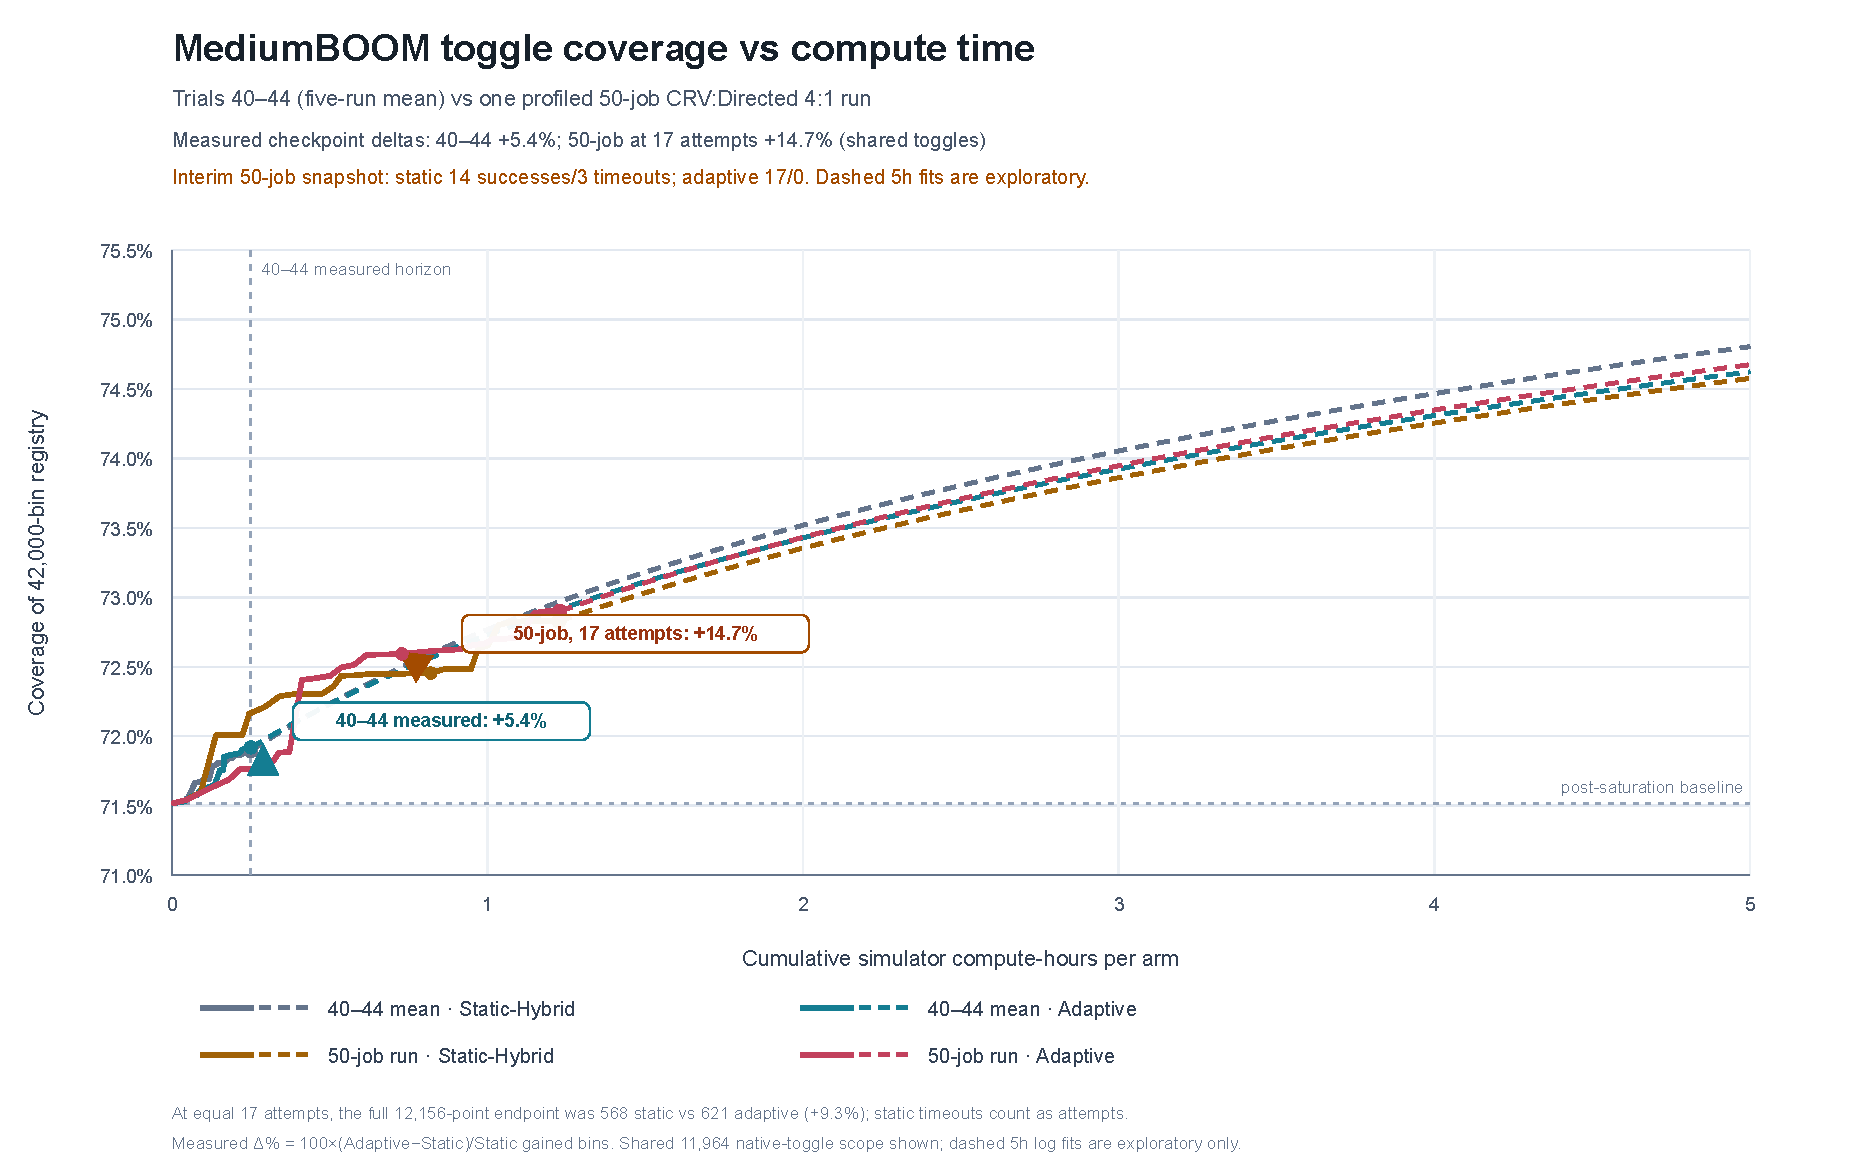
\includegraphics[width=0.92\textwidth]{adaptive_vs_static_post_saturation.pdf}
\caption{Resource allocation and coverage. (a) The separate five-slot trace is illustrative, not part of the reported 95\% CRV/directed evaluation. (b) Post-saturation coverage versus compute-hours: trials 40--44 are the five-trial mean to 0.25 hours (+5.4\% Adaptive); the 50-job run shows the interim equal-17-attempt checkpoint (+14.7\%, 453 versus 395 bins). Five-hour log continuations are exploratory projections, not observed outcomes, and may cross.}
\label{fig:allocation-and-coverage}
\end{figure*}

The five-pair subset is exploratory; its 200-catalog log values are projections, not observed Compute95. The toggle catalog has no formal jobs, so these data neither establish proof-based closure nor a reliable general policy advantage. Initialization cost, job duration, and feedback delay remain potential explanations for observed differences.

\section{Conclusion}
ChiaLoop formulates verification work allocation as repeated decisions under an explicit objective, a frozen coverage universe, and constrained execution capacity. In five exploratory post-saturation MediumBOOM trial pairs at a 0.25 compute-hour checkpoint, Static-Hybrid accumulated 803 new-bin hits and Adaptive 846 (+8.6 per trial on average). Log projections to 200 catalogs suggest 11.09\% and 11.55\% additional residual-set closure; these values are exploratory projections, not measured outcomes.

\begin{thebibliography}{3}\footnotesize
\bibitem{masamba} N. Masamba, K. Eder, and T. Blackmore, ``Supervised learning for coverage-directed test selection in simulation-based verification,'' in \emph{Proc. IEEE Int. Conf. Artificial Intelligence Testing (AITest)}, 2022, pp. 19--25, doi: 10.1109/AITest55621.2022.00012.
\bibitem{chia} A. Cui \emph{et al.}, ``CHIA: An open-source framework for principled, agentic AI-driven hardware/software co-design research,'' arXiv:2606.27350, 2026. [Online]. Available: \url{https://arxiv.org/abs/2606.27350}
\bibitem{boom} C. Celio, D. A. Patterson, and K. Asanovi\'{c}, ``The Berkeley Out-of-Order Machine (BOOM): An industry-competitive, synthesizable, parameterized RISC-V processor,'' Univ. California, Berkeley, Tech. Rep. UCB/EECS-2015-167, Jun. 2015.
\end{thebibliography}
\end{document}
